\documentclass[9pt]{beamer}
%\usetheme[background=light]{metropolis}
\usetheme{Warsaw}
%\usefonttheme{professionalfonts}
\usefonttheme{serif}
\usepackage{fontspec}
\usepackage{media9}
\usepackage{tikz}
\usepackage[utf8]{inputenc}
\usepackage{amsmath}
\usepackage{algorithm}
\usepackage[noend]{algpseudocode}

\usetikzlibrary{shapes,snakes}
%\usefonttheme{structurebold}
\usecolortheme{dove}
\setmainfont{Georgia}

\setbeamertemplate{headline}{%
\leavevmode%
  \hbox{%
    \begin{beamercolorbox}[wd=\paperwidth,ht=5.8ex,dp=1.125ex]{palette}%
        \insertsectionnavigationhorizontal{\paperwidth}{}{\hskip0pt plus1filll}
    \end{beamercolorbox}%
  }
}


\setbeamertemplate{section in head/foot}{%
    \if\insertsectionheadnumber1
        \tikz\node[draw=black,fill=black,shape=signal,text=white]{\insertsectionhead\hskip.3cm};
    \else
        \tikz\node[draw=black,fill=black,shape=signal,signal from=west, signal to=east,text=white]     {\insertsectionhead\hskip.3cm};
  \fi
}

\setbeamertemplate{section in head/foot shaded}{%
    \if\insertsectionheadnumber1
        \tikz\node[draw=black,fill=white,shape=signal,text=black]{\insertsectionhead\hskip.3cm};
    \else
        \tikz\node[draw=black,fill=white,shape=signal,signal from=west, signal to=east,text=black]     {\insertsectionhead\hskip.3cm};
  \fi
}

\setbeamerfont{section in head/foot}{size=\fontsize{4}{6}\selectfont}

\title{Whirlpool}
\subtitle{Data Acquisition using N-node Distributed Web Crawler}
\author{Rihan Pereira, MSCS}
\institute[California State University Channel Islands]
{
%  %\inst{1}%
  \textit{Advisor:} Dr. Michael Soltys\\
  Department of Computer Science \\
  MSCS Graduate 2018-2019
}

\titlegraphic{\includegraphics[width=.3\textwidth,height=.2\textheight]{../csuci-mscs-thesis-dist-web-crawler/media/correctlogo.jpg}~}
\date{\today}
\usepackage{picture}
\begin{document}

% real meat of the presentation
% -------------------------------------
\begin{frame}[plain]
  \titlepage
\end{frame}

% table of contents a.k.a outline
% -------------------------------------
\begin{frame}[plain]
  %\frametitle{Agenda}
  %\tableofcontents[hideallsubsections]
  \begin{itemize}[<+->]
  \item Motivation \& Contributions
  \item Crawler characteristics \& history
  \item Mercator 1999 (Heydon \& Najork)
  \item Software Design Principles
    \makebox(0,0){\put(40,5.3\normalbaselineskip){%
               $\left.\rule{0pt}{2.3\normalbaselineskip}\right\}$ background}}
  \item Whirlpool: Event driven architecture
  \item Whirlpool: Fetcher
  \item Whirlpool: Parser
  \item Whirlpool: Deduplication
  \item Whirlpool: Distributed Crawling
  \item Whirlpool: Operations
    \makebox(0,0){\put(57,10.5\normalbaselineskip){%
               $\left.\rule{0pt}{4.1\normalbaselineskip}\right\}$ implementation \& results}}
  \item Future work
  \end{itemize}
  
\end{frame}

\section[Motiv. \& Contrib]{Motivation \& Contribution}
\begin{frame}[plain]
  \centering{Motivation \& Contribution}
\end{frame}

% -------------------------------------

\begin{frame}{Motivation}
  \centering
  \includegraphics[width=8cm, height=6cm, keepaspectratio]{../csuci-mscs-thesis-dist-web-crawler/media/crawler/data_hierarchy.png}
  \pause
  \\
  Self-actualization (AI) is great, but you first need food, water, and shelter (data literacy, collection, and infrastructure).”
\end{frame}

% -------------------------------------

\begin{frame}{Contributions}
  to be completed
\end{frame}

% -------------------------------------

\section[Crawler history]{Crawler characteristics \& history}
\begin{frame}[plain]
  \centering{Crawler characteristics \& history}
\end{frame}

% -------------------------------------

\begin{frame}{Coverage \& Freshness}
  \centering
  \includegraphics[width=10cm, height=6cm, keepaspectratio]{../csuci-mscs-thesis-dist-web-crawler/media/crawler/crawl-ordering.png}
\end{frame}

% -------------------------------------

\begin{frame}{Seedlist}
  \begin{columns}[t]
    \column{.5\textwidth}
    \centering
    
\includegraphics[width=2.5cm,height=2cm]{img/monster.png}\\
    
\includegraphics[width=2.5cm,height=2cm]{img/dice.jpg}\\
    
\includegraphics[width=2.5cm,height=2cm]{img/ziprecruiter.png}
    \column{.5\textwidth}
    \centering
    
\includegraphics[width=2.5cm,height=2cm]{img/glassdoor.jpg}\\
    
\includegraphics[width=2.5cm,height=2cm]{img/indeed.png}\\
    
\includegraphics[width=2.5cm,height=2cm]{img/simplyhired.jpg}
  \end{columns}
\end{frame}

% -------------------------------------

\begin{frame}{Web crawlers (1990 - 2019)}
  \begin{figure}
    %\caption{Web crawlers timeline}
    \centering
    \resizebox{\linewidth}{!}{% Resize table to fit within

      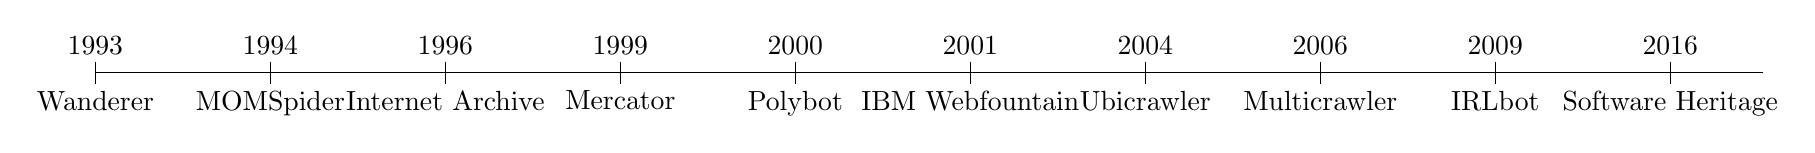
\begin{tikzpicture}[]
        % draw horizontal line
        \draw (0,0) -- (36/1.7,0);
        % draw vertical lines
        %\foreach \x in {0, 8, 15, 22, 29, 36, 41}{
        \foreach \x in {0, 4, 8, 12, 16, 20, 24, 28, 32, 36}{
          \draw (\x/1.8,4pt) -- (\x/1.8,-4pt);
        }
        % draw nodes
        \draw (0,0) node[below=3pt] { Wanderer } node[above=3pt] { 1993  };
        \draw (4/1.8,0) node[below=3pt] { MOMSpider } node[above=3pt] { 1994 };
        \draw (8/1.8,0) node[below=3pt] { Internet Archive } node[above=3pt] { 1996 };
        \draw (12/1.8,0) node[below=3pt] { Mercator } node[above=3pt] { 1999 };
        \draw (16/1.8,0) node[below=3pt] { Polybot } node[above=3pt] { 2000 };
        \draw (20/1.8,0) node[below=3pt] { IBM Webfountain } node[above=3pt] { 2001 };
        \draw (24/1.8,0) node[below=3pt] { Ubicrawler } node[above=3pt] { 2004 };
        \draw (28/1.8,0) node[below=3pt] { Multicrawler } node[above=3pt] { 2006 };
        \draw (32/1.8,0) node[below=3pt] { IRLbot } node[above=3pt] { 2009 };
        \draw (36/1.8,0) node[below=3pt] { Software Heritage } node[above=3pt] { 2016 };
      \end{tikzpicture}
    }
    \label{fig:time_line}
  \end{figure}
\end{frame}

% -------------------------------------

\section[Mercator]{Mercator 1999 (Heydon \& Najork)}
\begin{frame}[plain]
  \centering{Mercator 1999 (Heydon \& Najork)}
\end{frame}

% -------------------------------------

\begin{frame}{basic crawling algorithm}
  \begin{algorithm}[H]
    \begin{algorithmic}[1]
      \State $\text{Let I} \gets \text{\{1,2,3,4,5\}} \text{ such that seed set S = \{} U_i \text{| i } \in \text{I\}}$
      \State $U_f \gets \text{S; where } U_f \text{ is a Frontier queue}$
      \Procedure{Spider}{$U_f$}
      \While {$U_f \neq \emptyset$}
      \State $u \gets \text{Pop}(U_f)$ 
      \State $p \gets \text{Fetch}(u)$
      \State $T \gets \exists p\text{ [\{Extract}(p, t) \text{ | } t \text{ is a text \}]}$
      \State $L \gets \exists p\text{ [\{Extract}(p, l) \text{ | } l \text{ is a link \}]}$
      \State $U_f \gets U_f \cup L$
      \State $\exists u\text{ [\{Delete}(U_f, u) \text{ | } u \text{ is a already fetched URL\}]}$
      \EndWhile
      \EndProcedure
      \State \textbf{end}
    \end{algorithmic}
  \end{algorithm}
\end{frame}

% -------------------------------------

\begin{frame}{Mercator background}
  \centering
  \begin{figure}
  \includegraphics[width=10cm, height=6cm, keepaspectratio]{../csuci-mscs-thesis-dist-web-crawler/media/crawler/basic-crawler-architecture-v2.png}
  \caption{Mercator building blocks (Heydon \& Najork)}
  \end{figure}
\end{frame}

% -------------------------------------

\begin{frame}{Mercator: URL filter}
  \centering
  \begin{figure}
  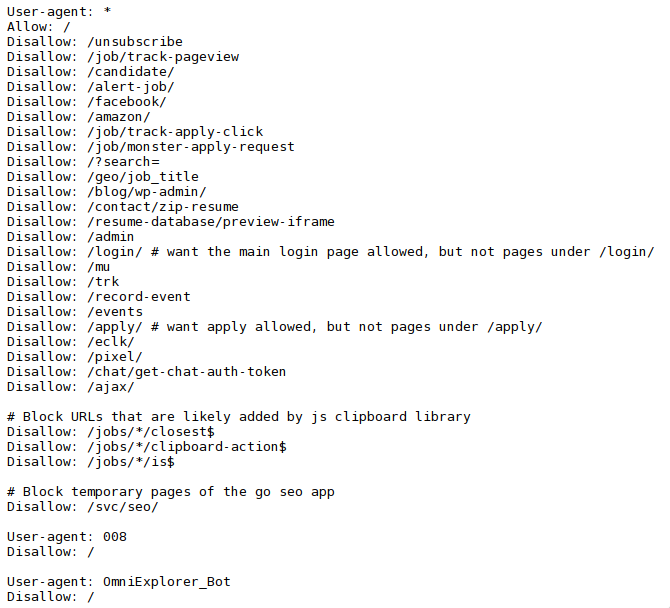
\includegraphics[width=8cm, height=12cm, keepaspectratio]{img/robots.png}
  %\caption{Mercator building blocks (Heydon \& Najork)}
  \end{figure}
\end{frame}

% -------------------------------------

\begin{frame}{URL Frontier Scheme}
  \centering
  \includegraphics[width=7cm, height=7.5cm, keepaspectratio]{../csuci-mscs-thesis-dist-web-crawler/media/crawler/url-frontier.png}
\end{frame}

% -------------------------------------

\begin{frame}{Front queue (Frontier Queue)}
  \centering
  \includegraphics[width=7cm, height=8cm, keepaspectratio]{../csuci-mscs-thesis-dist-web-crawler/media/crawler/f-queue.png}
\end{frame}

% -------------------------------------

\begin{frame}{Back queue (Frontier Queue)}
  \centering
  \includegraphics[width=8cm, height=9cm, keepaspectratio]{../csuci-mscs-thesis-dist-web-crawler/media/crawler/b-queue.png}
\end{frame}

% -------------------------------------

\section[Soft. design]{Software Design Principles}
\begin{frame}[plain]
  \centering{Software Design Principles}
\end{frame}

% -------------------------------------

\begin{frame}{Designing scalable systems}
  \begin{itemize}
    \pause
  \item Adding identical copies of components
    \pause
  \item Functional partitioning
    \begin{figure}
      \centering{\includegraphics[width=70mm, height=40mm, scale=0.1]{../csuci-mscs-thesis-dist-web-crawler/media/crawler/netflix.png}}
    \end{figure}
    \pause
  \item Data partitioning
  \end{itemize}
\end{frame}

% -------------------------------------

\begin{frame}{State Management}
  \only<1>{
    \centering{
      \begin{figure}
        \includegraphics[width=5cm, height=3cm, scale=1.3]{../csuci-mscs-thesis-dist-web-crawler/media/crawler/multi-cache-wrng.png}
        \caption{identical copies of same cached object}
      \end{figure}
    }
  }\only<2>{
    \centering{
      \begin{figure}
        \includegraphics[width=6cm, height=2cm, scale=0.1]{../csuci-mscs-thesis-dist-web-crawler/media/crawler/wrng-local-locks.png}
        \caption{Using local locks to access shared resources}
      \end{figure}
    }
  }\only<3>{
    \centering{
      \begin{figure}
        \includegraphics[width=6cm, height=2cm, scale=0.1]{../csuci-mscs-thesis-dist-web-crawler/media/crawler/rght-shared-locks.png}
        \caption{using shared locks to access shared resources}
      \end{figure}
    }
  }
\end{frame}

% -------------------------------------

\section[Event-driven]{Whirlpool: Event-driven architecture}
\begin{frame}[plain]
  \centering{Whirlpool: Event-driven architecture}
\end{frame}

% -------------------------------------

\begin{frame}{Message buses}
  \begin{columns}[t]
    \column{.5\textwidth}
    \centering
    
\includegraphics[width=4cm,height=2cm]{img/rmq.png}\\
    \vrule{}
    \column{.5\textwidth}
    \centering
    
\includegraphics[width=4.3cm,height=2.7cm]{img/kafka.png}\\
  \end{columns}
\end{frame}

% -------------------------------------

\begin{frame}{Message Queue(MQ)}
  \begin{columns}
    \column{0.7\textwidth}
    \centering{
      \includegraphics[width=8cm, height=6cm, keepaspectratio]{../csuci-mscs-thesis-dist-web-crawler/media/crawler/mq_basic.png}
    }
    \column{0.4\textwidth}
    \begin{itemize}
      \pause
    \item decoupling
      \pause
    \item scaled independently
      \pause
     \item balancing traffic
       \pause
     \item fault-tolerance
    \end{itemize}
  \end{columns}
  
\end{frame}

% -------------------------------------

\begin{frame}{MQ: Routing mechanisms}
  \begin{itemize}
    \pause
  \item Direct Worker Queue Data Flow
    \pause
  \item Fanout
    \pause
  \item Topic
    \pause
  \item Header
  \end{itemize}
\end{frame}

% -------------------------------------

\begin{frame}{Direct Worker Queue Data Flow}
  \centering
  \includegraphics[width=7cm, height=8cm, keepaspectratio]{../csuci-mscs-thesis-dist-web-crawler/media/crawler/rmq-broker.png}
\end{frame}

% -------------------------------------

\begin{frame}{RabbitMQ: Message bus}
  \centering
  \includegraphics[width=10cm, height=6cm, keepaspectratio]{../csuci-mscs-thesis-dist-web-crawler/media/crawler/multi-container-deploy.png}
\end{frame}

% -------------------------------------

\begin{frame}{Language runtime}
  %\begin{columns}[t]
    %\column{.2\textwidth}
  \begin{figure}
    \centering
    
\includegraphics[width=2.5cm,height=2cm]{img/javalogo.jpg}
    
\includegraphics[width=2.5cm,height=2cm]{img/pylogo1.png}\\
    
\includegraphics[width=2.5cm,height=2cm]{img/jslogo.png}
    
\includegraphics[width=2.5cm,height=2cm]{img/javalogo.jpg}
  \end{figure}
    %\column{.2\textwidth}
    %\centering
  %\end{columns}
  \centering
\end{frame}

% -------------------------------------

\begin{frame}{development vs. production docker containers}
  \only<1>{
    \centering{
      \begin{figure}
        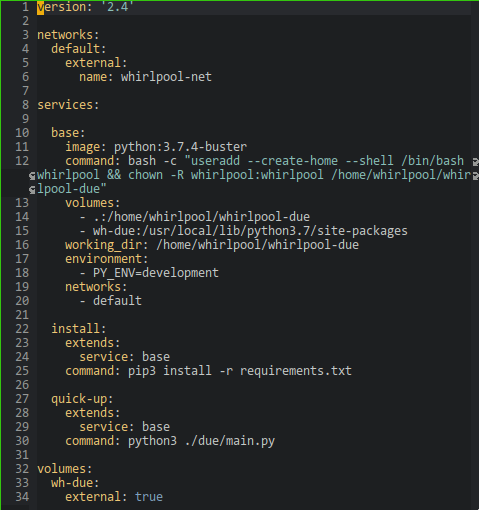
\includegraphics[width=6.5cm,height=7.5cm]{img/dockerdev.png}
      \end{figure}
    }
  }\only<2>{
    \centering{
      \begin{figure}
        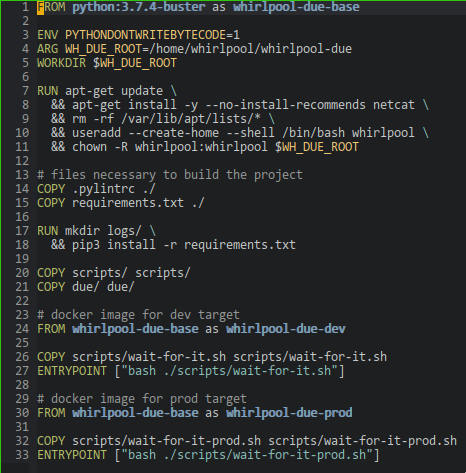
\includegraphics[width=6.5cm,height=7.5cm]{img/dockerfile.png}
      \end{figure}
    }
  }
  %\only<3>{
  %  \centering{
  %    \begin{figure}
  %      
  %    \end{figure}
  %  }
  %}
\end{frame}

% -------------------------------------

\begin{frame}{development vs. production docker containers}
  \centering
  \includemedia[
  width=6.5cm,
  height=7.5cm,
  activate=pageopen,
  addresource=img/dockercompose.mp4,
  flashvars={
    %important: same path as in `addresource'
    source=img/dockercompose.mp4
    &autoPlay=true
    &loop=true
    &scaleMode=letterbox
  }
]{}{VPlayer.swf}
\end{frame}

% -------------------------------------

\section[Fetcher]{Whirlpool: Fetcher}
\begin{frame}[plain]
  \centering{Whirlpool: Fetcher}
\end{frame}

% -------------------------------------

\begin{frame}{Whirlpool: Fetcher}
  \centering
  \includegraphics[width=12cm, height=7cm, keepaspectratio]{../csuci-mscs-thesis-dist-web-crawler/media/crawler/dns_response_time.png}
\end{frame}

% -------------------------------------

\section[Parser]{Whirlpool: Parser}
\begin{frame}[plain]
  \centering{Whirlpool: Parser}
\end{frame}

% -------------------------------------

\begin{frame}{Parser}
  \centering
  \includegraphics[width=10cm, height=6cm, keepaspectratio]{../csuci-mscs-thesis-dist-web-crawler/media/crawler/docparsers.png}
\end{frame}

% -------------------------------------

\section[Dedupe]{Whirlpool: Deduplication}
\begin{frame}[plain]
  \centering{Whirlpool: Deduplication}
\end{frame}

% -------------------------------------

\begin{frame}{Fingerprinting}
  \begin{figure}
    \centering
    \includegraphics[width=11.5cm,height=2.5cm]{../csuci-mscs-thesis-dist-web-crawler/media/crawler/fingerprinting.png}
  \end{figure}
\end{frame}

% -------------------------------------

\begin{frame}{Bloom filter}
  
\end{frame}

% -------------------------------------

\begin{frame}{Shingling: Near Deduplication}
  \pause
  \begin{itemize}
  \item gather analyze design develop and test applications using agile methodology
  \item using agile methodology gather analyze design develop and test applications
  \end{itemize}
  \pause
  \begin{figure}
    \centering
    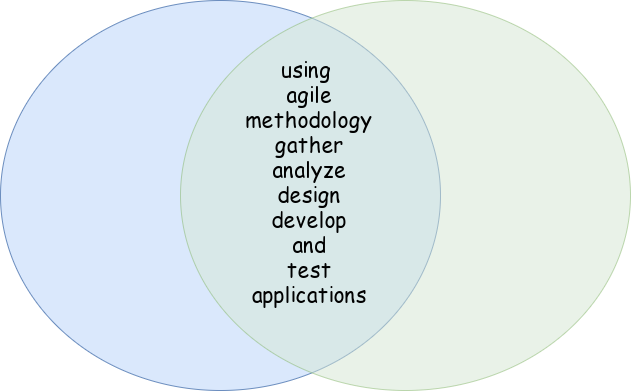
\includegraphics[width=9.5cm,height=4.5cm]{img/bagofwords.png}
  \end{figure}
\end{frame}

% -------------------------------------

\begin{frame}{Shingling: Near Deduplication}
  \begin{itemize}
  \item gather analyze design develop and test applications using agile methodology
  \item As per google trends Typescript to be among the popular programming languages in the next five years
  \end{itemize}
  \pause
  \begin{figure}
    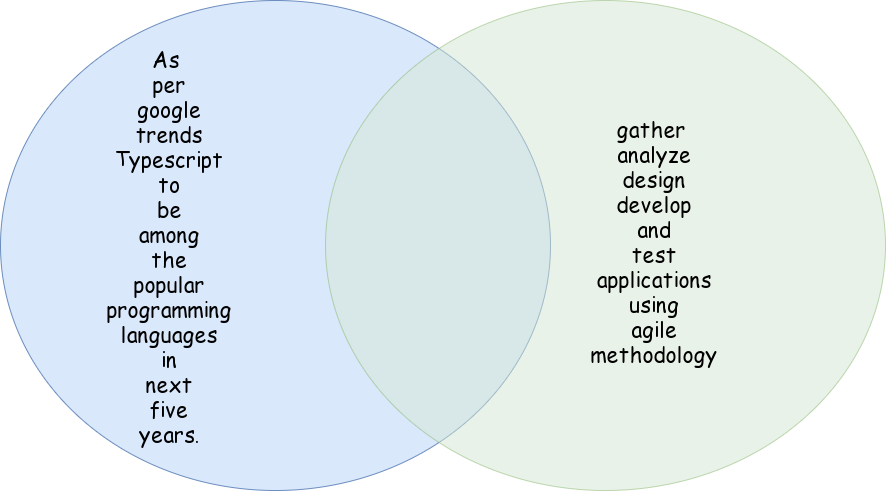
\includegraphics[width=9.5cm,height=4.5cm]{img/bagofwordsintersect.png}
  \end{figure}
\end{frame}

% -------------------------------------

\begin{frame}{Shingling: Near Deduplication}
  \begin{itemize}
  \item Here are the next top five programming languages in coming years according to google trends
  \item As per google trends Typescript to be among the popular programming languages in the next five years
  \end{itemize}
  \pause
  \begin{figure}
    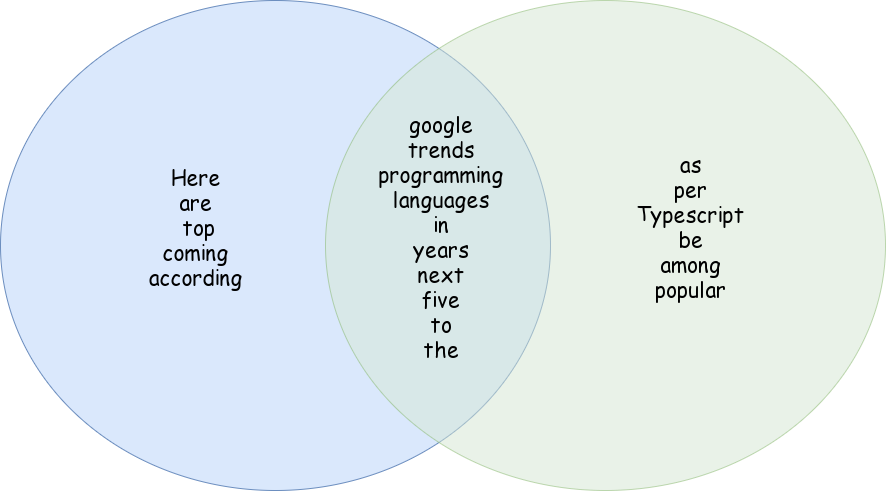
\includegraphics[width=9.5cm,height=4.5cm]{img/bagofwordsintersect2.png}
  \end{figure}
\end{frame}

% -------------------------------------

\begin{frame}{Shingling: Near Deduplication}
  \begin{itemize}
  \item gather analyze design develop and test applications using agile methodology
  \item using agile methodology gather analyze design develop and test applications
  \end{itemize}
  \pause
  \begin{figure}
    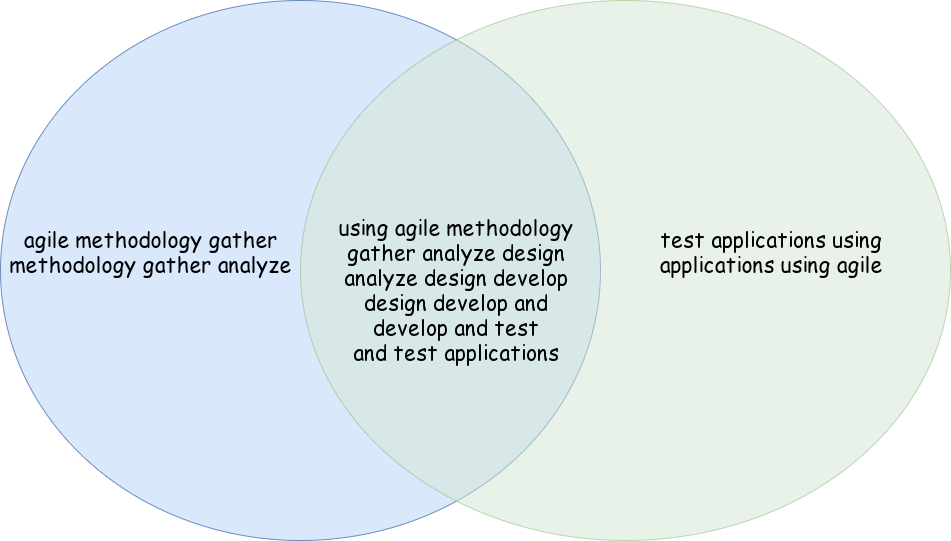
\includegraphics[width=9.5cm,height=4.5cm]{img/shinglesintersect1.png}
  \end{figure}
\end{frame}

% -------------------------------------

\begin{frame}{Shingling: Near Deduplication}
  \begin{itemize}
  \item Here are the next top five programming languages in coming years according to google trends
  \item As per google trends Typescript to be among the popular programming languages in the next five years
  \end{itemize}
  \pause
  \begin{figure}
    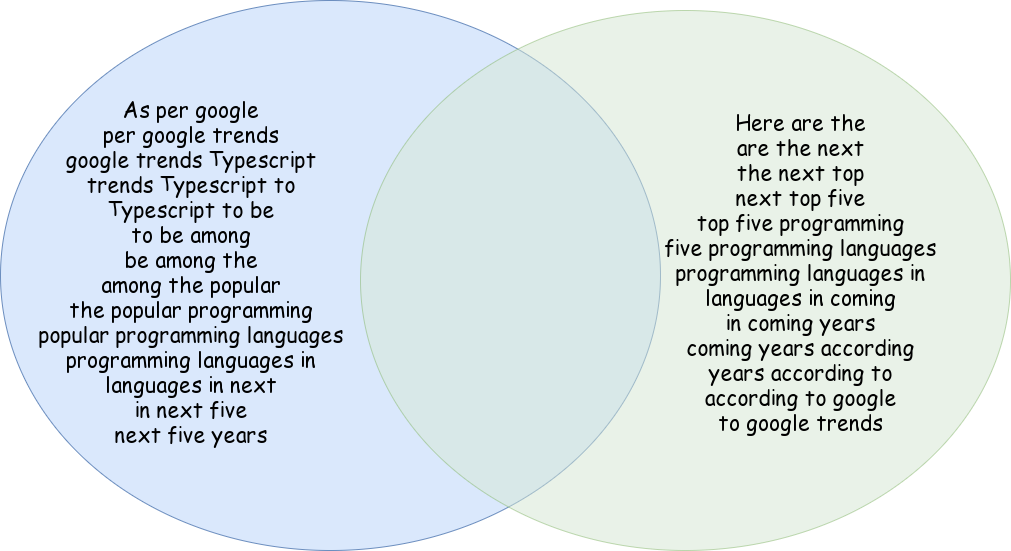
\includegraphics[width=9.5cm,height=4.5cm]{img/shinglesintersect2.png}
  \end{figure}
\end{frame}

% -------------------------------------

\begin{frame}{Shingling: Near Deduplication}
  \only<1>{
    \centering {
      \begin{figure}
      
\includegraphics[width=8cm,height=2cm]{../csuci-mscs-thesis-dist-web-crawler/media/crawler/monster.png}
      \end{figure}
      \begin{figure}
      
\includegraphics[width=8cm,height=2cm]{../csuci-mscs-thesis-dist-web-crawler/media/crawler/simplyhired.png}
      \end{figure}
      \begin{figure}
      
\includegraphics[width=8cm,height=2cm]{../csuci-mscs-thesis-dist-web-crawler/media/crawler/dice.png}
      \end{figure}
    }
  }\only<2>{
    \centering {
      \begin{figure}
        \includegraphics[width=11cm,height=3cm]{../csuci-mscs-thesis-dist-web-crawler/media/crawler/shingles.png}
      \end{figure}
    }
  }
\end{frame}

% -------------------------------------

\begin{frame}{Locality Sensitive Hashing}
  
\end{frame}

% -------------------------------------

\section[Dist. Crawl]{Whirlpool: Distributed Crawling}
\begin{frame}[plain]
  \centering{Whirlpool: Distributed Crawling}
\end{frame}

% -------------------------------------

\begin{frame}{Host splitting in Mercator}
  \begin{figure}
    \centering 
    \includegraphics[width=10cm, height=5cm, keepaspectratio]{../csuci-mscs-thesis-dist-web-crawler/media/crawler/host-splitterv3.png}
  \end{figure}

  \begin{figure}
    \centering
    \includegraphics[width=6cm,height=1cm]{../csuci-mscs-thesis-dist-web-crawler/media/crawler/requestboundaries.png}
  \end{figure}
\end{frame}

% -------------------------------------

\begin{frame}{Rebalancing: mod N}
  \only<1>{
    \centering {
      \begin{figure}
      \includegraphics[width=8cm,height=3cm]{../csuci-mscs-thesis-dist-web-crawler/media/crawler/modnsplit.png}
      \end{figure}
    }
  }\only<2>{
    \centering {
      \begin{figure}
        \includegraphics[width=10cm,height=3cm]{../csuci-mscs-thesis-dist-web-crawler/media/crawler/modn_info.png}
      \end{figure}
    }
  }
\end{frame}

% -------------------------------------

\begin{frame}{Rebalancing: virtual nodes}
  \only<1>{
    \centering {
      \begin{figure}
      \includegraphics[width=8cm,height=3cm]{../csuci-mscs-thesis-dist-web-crawler/media/crawler/vnodesplit1.png}
      \end{figure}
    }
  }\only<2>{
    \centering {
      \begin{figure}
     \includegraphics[width=8cm,height=3cm]{../csuci-mscs-thesis-dist-web-crawler/media/crawler/vnodesplit2.png}
      \end{figure}
    }
  }\only<3>{
    \centering {
      \begin{figure}
     \includegraphics[width=8cm,height=2cm]{../csuci-mscs-thesis-dist-web-crawler/media/crawler/addingnode.png}
      \end{figure}
    }
  }
\end{frame}

% -------------------------------------

\begin{frame}{Zookeeper}
  \begin{columns}[t]
    \column{.5\textwidth}
    \begin{figure}
     \centering \includegraphics[width=5cm,height=2cm]{../csuci-mscs-thesis-dist-web-crawler/media/crawler/zookeeper.png}
   \end{figure}
   \column{.5\textwidth}
   \begin{figure}
     \centering
     \includegraphics[width=5cm,height=2.5cm]{../csuci-mscs-thesis-dist-web-crawler/media/crawler/zookeeper_info.png}
   \end{figure}
 \end{columns}
\end{frame}

% -------------------------------------

\section[opswork]{Whirlpool: Operations}
\begin{frame}[plain]
  \centering{Whirlpool: Operations}
\end{frame}

% -------------------------------------

\subsection{From 10,000 ft.}
\begin{frame}{From 10,000 ft.}
 \centering
 \includegraphics[width=10cm, height=8cm, keepaspectratio]{../csuci-mscs-thesis-dist-web-crawler/media/crawler/ten-thousand-feet-aws.png} 
\end{frame}

% -------------------------------------

\subsection{From 5,000 ft.}
\begin{frame}{From 5,000 ft.}
  \centering
  \includegraphics[width=10cm, height=8cm, keepaspectratio]{../csuci-mscs-thesis-dist-web-crawler/media/crawler/aws-deploy-5k-feet.png}
\end{frame}

% -------------------------------------

\begin{frame}{Infrastructure as a code}
  \centering
  \includemedia[
  width=6.5cm,
  height=7.5cm,
  activate=pageopen,
  addresource=img/cf.mp4,
  flashvars={
    %important: same path as in `addresource'
    source=img/cf.mp4
    &autoPlay=true
    &loop=true
    &scaleMode=letterbox
  }
]{}{VPlayer.swf}
\end{frame}

% -------------------------------------

\begin{frame}{Recap}
  \begin{itemize}
  \item Microservices
  \item Load balancing
  \item Decoupling
  \item Extensible
  \item Distributed Systems(Partitioning)
  \item Logging \& metrics calculation
  \item Fault tolerance
  \item Resiliency
  \end{itemize}
\end{frame}

% -------------------------------------

\section[Future]{Future work}
\begin{frame}[plain]
  \centering{Future work}
\end{frame}

% -------------------------------------

\begin{frame}{future work}
  \only<1>{
    \centering {
      Indexing crawled data \& logs using Elasticsearch
      \begin{figure}
        \includegraphics[width=3.0cm,height=1.5cm]{img/es.png}
      \end{figure}
    }
  }\only<2>{
    \centering {
      Adding comprehensive coverage
      \begin{figure}
      \includegraphics[width=9cm,height=5cm]{../csuci-mscs-thesis-dist-web-crawler/media/crawler/crawl-ordering.png}
    \end{figure}
  }
}\only<3>{
  \centering {
    Content Extraction
  }
}\only<4>{
    \centering {
      Categorizing Jobs using ML algorithm
    }
  }\only<5>{
    \centering {
      SeenTest: Inserting and Querying Simhashes using LSH
    }
  }\only<6>{
    \begin{columns}[t]
      \column{.3\textwidth}
      \centering
      \includegraphics[width=1cm,height=1cm]{img/kub.png}
      \column{.5\textwidth}
      Deploying whirlpool using kubernetes
    \end{columns}
    \begin{figure}
      \centering
      \includegraphics[width=11cm,height=4cm]{img/kubgraph.png}
    \end{figure}
}
\end{frame}

% -------------------------------------

%\section{Demo}
%\begin{frame}{Demo}
%  
%\end{frame}

% -------------------------------------

\begin{frame}[plain]
  \centering{Thank you! Questions ?}
\end{frame}
\end{document}
%%% Local Variables:
%%% mode: latex
%%% TeX-master: t
%%% End:
